\documentclass[12pt]{article}
\linespread{1.2}
\usepackage[margin=2cm]{geometry}
\usepackage[utf8]{inputenc}
\usepackage{amsfonts}
\usepackage{amsmath}
\usepackage{multicol}
\usepackage{amsthm}
\usepackage{amssymb,scrextend}
\usepackage{graphicx,tikz,pgfplots}
\usetikzlibrary{arrows}
\pgfplotsset{compat=1.18}
\newtheorem{dfn}{Definition}
\renewcommand{\qed}{\hfill$\blacksquare$}
\let\newproof\proof
\renewenvironment{proof}{\vspace{1em}\begin{addmargin}[2em]{0em}\begin{newproof}}{\end{newproof}\end{addmargin}\qed}
\newenvironment{theorem}[2][Theorem]{\begin{trivlist}
\item[\hskip \labelsep {\bfseries #1} \hskip \labelsep {\bfseries #2.}]}{\end{trivlist}}
\newenvironment{example}[2][Example]{\begin{trivlist}
\item[\hskip \labelsep {\bfseries #1} \hskip \labelsep {\bfseries #2.}]}{\end{trivlist}}
\newenvironment{lemma}[2][Lemma]{\begin{trivlist}
\item[\hskip \labelsep {\bfseries #1} \hskip \labelsep {\bfseries #2.}]}{\end{trivlist}}
\newenvironment{exercise}[2][Exercise]{\begin{trivlist}
\item[\hskip \labelsep {\bfseries #1} \hskip \labelsep {\bfseries #2.}]}{\end{trivlist}}
\newenvironment{problem}[2][Problem]{\begin{trivlist}
\item[\hskip \labelsep {\bfseries #1} \hskip \labelsep {\bfseries #2.}]}{\end{trivlist}}
\newenvironment{corollary}[2][Corollary]{\begin{trivlist}
\item[\hskip \labelsep {\bfseries #1} \hskip \labelsep {\bfseries #2.}]}{\end{trivlist}}
\usepackage{fancyhdr,enumitem,changepage,url}
\pagestyle{fancy}
\author{Warren Atkison}
\date{\today}
\setlength{\headheight}{15pt}
\begin{document}
\fancyhf{}
\fancyhead[L]{Warren Atkison}
\fancyhead[C]{Homework Set 3}
\fancyhead[R]{\today}
\fancyfoot[R]{\thepage}

\subsection*{Experiment: The Transition to Chaos}
	You are to compute the orbit of 0 under $Q_c(x) = x^2 + c$ for at
least 50 different $c$-values as specified below. For each such $c$, the goal is to
record the ultimate or “asymptotic” behavior of the orbit of 0. This means
that we are only interested in what eventually happens to the orbit of 0. Is it
attracted to a fixed point? To a $k$-cycle? Is there no pattern to the orbit at
all?

\begin{center}
	\includegraphics[scale = .24]{Fig3.6.jpg}
\end{center}

From $-0.75 < c < 0.25$, the orbit of zero is attracted to a fixed point, then from $-1.25 < c < -0.75$ the orbit is attracted to a 2-cycle, from $-1.4 < c < -1.25$ the orbit is attracted to a 4-cycle or 8-cycle, from $-1.78 < c < -1.76$ there are some 3 and 6 cycles, and from $-2 < -1.78$ and $-1.75 < c < -1.4$ there is no pattern, just chaos!

\begin{exercise}{1} 
	Each of the following functions undergoes a bifurcation of fixed points at
the given parameter value. In each case, use algebraic or graphical methods to
identify this bifurcation as either a saddle-node or period-doubling bifurcation,
or neither of these. In each case, sketch the phase portrait for typical parameter
values below, at, and above the bifurcation value.
\begin{itemize}
	\item[a.] $F_{\lambda}(x) = x + x^2 + \lambda,~ \lambda = 0$
		\begin{center}
			\begin{tikzpicture}[scale = 0.9]
				\begin{axis}[xmin = -2, xmax = 2, ymin = -2, ymax = 2, axis x line = middle, axis y line = middle]
					\addplot[domain=-2:2] {x};
					\addplot[domain=-2:2] {x + x^2};
				\end{axis}
			\end{tikzpicture}	
		\end{center}
		This is a period doubling bifurcation. 
		\begin{center}
				\begin{tikzpicture}[scale = 2]
				\draw[latex-] (-2.5,0) -- (2.5,0) ;
				\draw[-latex] (-2.5,0) -- (2.5,0) ;
				\foreach \x in  {-2,-1,0,1,2}
				\draw[shift={(\x,0)},color=black] (0pt,3pt) -- (0pt,-3pt);
				\foreach \x in {-2,-1,0,1,2}
				\draw[shift={(\x,0)},color=black] (0pt,0pt) -- (0pt,-3pt) node[below] 
				{$\x$};
				\draw[*-] (-0.04,0) -- (1,0);
				\draw[o-] (-1.04,0) -- (1,0);
				\draw[latex-] (0.5,0) -- (-1,0);
				\draw[latex-] (1.75,0) -- (-1,0);
				\draw[latex-] (-0.5,0) -- (-2,0);
				\draw[latex-] (-1.75,0) -- (1,0);

				
			\end{tikzpicture}
		\end{center}
	\item[b.] $F_{\lambda}(x) = x + x^2 + \lambda,~ \lambda = -1$
		\begin{center}
			\begin{tikzpicture}[scale = 0.9]
				\begin{axis}[xmin = -2, xmax = 2, ymin = -2, ymax = 2, axis x line = middle, axis y line = middle]
					\addplot[domain=-2:2] {x};
					\addplot[domain=-2:2] {x + x^2 - 1};
				\end{axis}
			\end{tikzpicture}	
		\end{center}
		This is a period doubling bifurcation. 
		\begin{center}
				\begin{tikzpicture}[scale = 2]
				\draw[latex-] (-2.5,0) -- (2.5,0) ;
				\draw[-latex] (-2.5,0) -- (2.5,0) ;
				\foreach \x in  {-2,-1,0,1,2}
				\draw[shift={(\x,0)},color=black] (0pt,3pt) -- (0pt,-3pt);
				\foreach \x in {-2,-1,0,1,2}
				\draw[shift={(\x,0)},color=black] (0pt,0pt) -- (0pt,-3pt) node[below] 
				{$\x$};
				\draw[*-] (0.96,0) -- (1,0);
				\draw[*-] (-1.04,0) -- (1,0);
				\draw[latex-] (0.5,0) -- (1,0);
				\draw[latex-] (1.5,0) -- (-1,0);
				\draw[latex-] (-0.5,0) -- (2,0);
				\draw[latex-] (-1.5,0) -- (-2,0);

				
			\end{tikzpicture}
		\end{center}
	\item[c.] $G_{\mu}(x) = \mu x + x^3,~ \mu = -1$
		\begin{center}
			\begin{tikzpicture}[scale = 0.9]
				\begin{axis}[xmin = -2, xmax = 2, ymin = -2, ymax = 2, axis x line = middle, axis y line = middle]
					\addplot[domain=-2:2] {x};
					\addplot[domain=-2:2] {-x + x^3};
				\end{axis}
			\end{tikzpicture}	
		\end{center}
		This is neither a period doubling or saddle-node bifurcation. 
		\begin{center}
				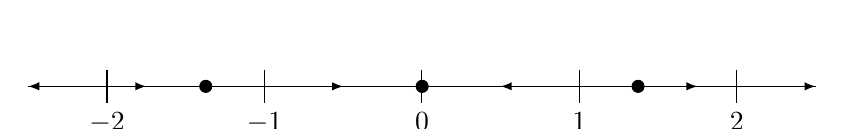
\begin{tikzpicture}[scale = 2]
				\draw[latex-] (-2.5,0) -- (2.5,0) ;
				\draw[-latex] (-2.5,0) -- (2.5,0) ;
				\foreach \x in  {-2,-1,0,1,2}
				\draw[shift={(\x,0)},color=black] (0pt,3pt) -- (0pt,-3pt);
				\foreach \x in {-2,-1,0,1,2}
				\draw[shift={(\x,0)},color=black] (0pt,0pt) -- (0pt,-3pt) node[below] 
				{$\x$};
				\draw[*-] (-0.04,0) -- (1,0);
				\draw[*-] (-1.414,0) -- (1,0);
				\draw[*-] (1.414,0) -- (1,0);
				\draw[latex-] (0.5,0) -- (1,0);
				\draw[latex-] (1.75,0) -- (-1,0);
				\draw[latex-] (-0.5,0) -- (-2,0);
				\draw[latex-] (-1.75,0) -- (-2,0);

				
			\end{tikzpicture}
		\end{center}

	\item[e.] $S_{\mu}(x) = \mu\sin x,~ \mu = 1$
		\begin{center}
			\begin{tikzpicture}[scale = 0.9]
				\begin{axis}[xmin = -2, xmax = 2, ymin = -2, ymax = 2, axis x line = middle, axis y line = middle]
					\addplot[domain=-2:2] {x};
					\addplot[domain=-2:2] {sin(deg(x))};
				\end{axis}
			\end{tikzpicture}	
		\end{center}
		This is neither a period doubling or saddle-node bifurcation. 
		\begin{center}
				\begin{tikzpicture}[scale = 2]
				\draw[latex-] (-2.5,0) -- (2.5,0) ;
				\draw[-latex] (-2.5,0) -- (2.5,0) ;
				\foreach \x in  {-2,-1,0,1,2}
				\draw[shift={(\x,0)},color=black] (0pt,3pt) -- (0pt,-3pt);
				\foreach \x in {-2,-1,0,1,2}
				\draw[shift={(\x,0)},color=black] (0pt,0pt) -- (0pt,-3pt) node[below] 
				{$\x$};
				\draw[*-] (-0.04,0) -- (1,0);
				\draw[latex-] (0.5,0) -- (1,0);
				\draw[latex-] (1.5,0) -- (1,0);
				\draw[latex-] (-0.5,0) -- (-2,0);
				\draw[latex-] (-1.5,0) -- (-2,0);

				
			\end{tikzpicture}
		\end{center}
\end{itemize}
\end{exercise}
\begin{exercise}{3}
	Prove that the cycle of period 2 given by the $q_{\pm}$ is attracting for $-5/4 < c < -3/4$ for $Q_c(x) = x^2 + c$
\end{exercise}
\begin{proof} First we find our prime period 2 points
	\begin{align*}
		Q_c^{2}(x) &= (x^2 + c)^2 + c = x^4 + 4cx^2 + c^2 + c = x \\
		\implies& x^4 + 4cx^2 - x + c^2 + c = (x^2 - x + c)(x^2 + x + c + 1) = 0 
	\end{align*}
	Since we want points of prime period 2, we solve for the roots of $x^2 + x + c + 1$.
	\begin{align*}
		x = \frac{-1 \pm \sqrt{1 - 4(c+1)}}{2} = \frac{-1 \pm \sqrt{-3-4c}}{2} = q
	\end{align*}
	Recall
	\begin{align*}
		(Q_c^{2})^{'}(x) &= Q_c^{'}(x_0)\cdot Q_c^{'}(x_1).
	\end{align*}
	So then
	\[
		Q_c^{'}(x) = 2x
	\]
	\begin{align*}
		(Q_c^{2})^{'}(q) &= 2\left(\frac{1 + \sqrt{-3 -4c}}{2}\cdot\frac{1 - \sqrt{-3 - 4c}}{2}\right) \\
				 &= (1 + \sqrt{-3 - 4c})(1 - \sqrt{-3 -4c}) \\
				 &= 1 - (-3 - 4c) = 4 + 4c
	\end{align*}
	For the 2-cycle to be attracting, we want $|(Q_c^2)^{'}(q)| < 1$. So
	\begin{align*}
		|4 + 4c| < 1 &\implies -1 < 4 + 4c < 1 \implies -5 < 4c < -3 \\
			     &\implies -\frac{5}{4} < c < -\frac{3}{4}
	\end{align*}
\end{proof}
\end{document}
